\section{Mittwoch}

\subsection{Lehrinhalte FOPT5}

\subsubsection{Notizen zu den Lehrinhalten FOPT5}

\begin{itemize}
    \item Grundlagen der Rechnernetze:
    \begin{itemize}
        \item Schichtenmodell
        \item Protokolle
        \item IP-Adressen und DNS-Namen
        \item Transportprotokolle TCP und UDP, Portnummern
    \end{itemize}
    \item Socket-Schnittstelle:
    \begin{itemize}
        \item Schicht5-Schicht4-Grenze
        \item Client-Server
    \end{itemize}
    \item Kommunikation über UDP:
    \begin{itemize}
        \item DatagramSocket, DatagramPacket
        \item Beachtung der Unzuverlässigkeit von UDP
        \item[] (wegen der Unzuverlässigkeit von UDP kann es sein, dass ein client hängen bleibt, weil nie die Antwort des Servers ankommt - deshalb kann ein Timeout über \code{setSoTimeout()}\footnote{
        ``setSoTimeout``: \url{https://docs.oracle.com/en/java/javase/21/docs/api/java.base/java/net/DatagramSocket.html#setSoTimeout(int)} - abgerufen 24.02.2024
        } gesetzt werden. Es wird dann eine \code{SocketTimeoutException} geworfen, falls das timeout vor dem receive eintritt).
    \end{itemize}
    \item Multicast-Kommunikation
    \item Kommunikation über TCP:
    \begin{itemize}
        \item Socket, ServerSocket, Klassen aus dem Package java.io
        \item[] (TCP ist datenstromorientiert - Sendeoperationen und Empfangsoperationen stehen nicht in einem $1:1$-Verhältnis, eine Sendeoperation kann mehrere Empfangsoperationen haben, mehrere Sendeoperationen können eine Empfangsoperation haben.\\
        Also muss man erkennen, was eine logische Dateneinheit ist.
        Deshalb hat der Kurs vereinbart, dass ein newline-symbol \textbf{\textbackslash{n}} genutzt wird, um Nachrichtengrenzen zu erkennen.
        Bei UDP ist das nicht notwendig, da UDP nachrichtenorientiert ist.)
    \end{itemize}
    \item Sequenzielle und parallele Server:
    \begin{itemize}
        \item Statische Parallelität
        \item Dynamische Parallelität
        \item Mischformen
    \end{itemize}
    \item RMI:
    \begin{itemize}
        \item Stub, Skeleton
        \item ``Kochrezept``:
        \begin{enumerate}
            \item Interface definieren (extends Remote, Methoden mit throws Remote Exception-Klausel deklarieren)
            \item Interface implementieren (extends UnicastRemoteObject, Konstruktoren müssen mit throws RemoteException deklariert sein)
            \item Server programmieren (Objekte von 2 erzeugen und bei der RMI-Registry anmelden)
            \item Client programmieren (Objekte - die Stubs - aus der Registry über Naming.lookup() holen, Casting auf das in Schritt 1 definierte Interface, Methoden aufrufen)
        \end{enumerate}
    \end{itemize}
    \item Parallelität bei RMI
    \item Wertübergabe für Parameter und Rückgabewerte:
    \begin{itemize}
        \item falls Objekte serialisierbar und nicht exportiert sind
    \end{itemize}
    \item Referenzübergabe für Parameter und Rückgabewerte:
    \begin{itemize}
        \item falls Objekte exportiert sind
    \end{itemize}
    \item MVP-Prinzip für verteilte Anwendungen
\end{itemize}

\subsection{Notizen}
Das Interface \code{AutoCloseable} wird u.a. für die Implementierung der UDPSocket\footnote{\cite[269, Listing 5.1]{Oec22}}/ TCPSocket\footnote{\cite[286, Listing 5.7]{Oec22}}-Klassen genutzt, um sie mit \textbf{try-with-resources} nutzen zu können.\\

\noindent
Objekte, die man mittels \code{bind()}/ \code{rebind()} in der RMI-Registry registriert, \textit{müssen} das \code{Remote}-Interface implementieren\footnote{
Das macht spätestens der Typ des zweiten formalen Parameters von bspw. \textit{rebind(name: String, obj: Remote)} deutlich, s. \url{https://docs.oracle.com/en/java/javase/21/docs/api/java.rmi/java/rmi/registry/Registry.html#rebind(java.lang.String,java.rmi.Remote)} - abgerufen 22.2.2024
}.

\begin{tcolorbox}
Objekte, die als Remote Objekte funktionieren sollen, \textit{müssen} exportiert sein: ``Server``-Objekte \textit{müssen} also bspw. von \code{UnicastRemoteObject} ableiten, genauso wie Objekte, die über Call-by-Reference verwendet werden sollen.\\

    \noindent
    Objekte, die lediglich als Call-By-Value verwendet werden, müssen mindestens \code{Serializable} implementieren, genauso wie Objekte, die zum späteren Zugriff (\textit{nicht} als remote Objekt) in der RMI-Registry gespeichert werden\footnote{
        siehe hierzu auch Abschnitt \ref{sec:refrmi}.
}
\end{tcolorbox}\\

\noindent
Wie das Ende eines Stroms bekanntgegeben wird, ist abhängig von der jeweiligen Methode der genutzten Inputklasse - so meldet \code{readLine} von \code{BufferedReader} bspw. \code{null}, wenn das Ende des Datenstroms erreicht ist, \code{read()}\footnote{
    ``Class FilterInputStream``: \url{https://docs.oracle.com/en/java/javase/21/docs/api/java.base/java/io/FilterInputStream.html#read()} - abgerufen 22.2.2024
} der Klasse \code{FilterInputStream} in dem Fall hingegen \code{-1}.\\

\noindent
\code{DataInputStream} zum lesen einfacher Datentypen, \code{ObjectInputStream} für das Deserialisieren primitiver Datentypen und von Objekten.\\

\noindent
Beispiel für das Lesen von primitiven Datentypen über einen \code{DataInputStream}:

\begin{minted}[mathescape,
    linenos,
    numbersep=5pt,
    gobble=2,
    frame=lines,
    framesep=2mm]{java}
    byte[] buffer = new byte[4];
    buffer[0] = 1;
    DataInputStream dis = new DataInputStream(
        new ByteArrayInputStream(buffer)
    );
    dis.readInt();
\end{minted}\\

Eine \code{EOFEException} wird geworfen, wenn für einen erwarteten Datentypen nicht genug Daten vorliegen.
Im Folgenden ein Beispiel für ein \code{readInt()} - der Input-Stream erwartet ein byte-array der Größe 4, es wird aber nur eins
der Größe 1 übergeben:

\begin{minted}[mathescape,
    linenos,
    numbersep=5pt,
    gobble=2,
    frame=lines,
    framesep=2mm]{java}
    DataInputStream dis = new DataInputStream(
        new ByteArrayInputStream(new byte[1])
    );
    dis.readInt(); // EOFException
\end{minted}\\

\noindent
Ein \code{DatagramPacket}, das man zum Empfangen benutzen kann, erstellt man über den Aufruf des Konstruktors

\begin{minted}[mathescape,
    numbersep=5pt,
    gobble=2,
    framesep=2mm]{java}
    DatagramPacket(byte[]buf, int length);
\end{minted}\\

Über ein \code{DatagramSocket}-Objekt schreibt man dann die empfangenen Daten über den Aufruf \code{receive(p: DatagramPacket)}\footnote{
``receive``: \url{https://docs.oracle.com/en/java/javase/21/docs/api/java.base/java/net/DatagramSocket.html#receive(java.net.DatagramPacket)} - abgerufen 20.2.2024
}.\\

Nachrichten über UDP werden immer in Form eines \code{DatagramPacket} konstruiert.

\noindent
Umwandeln eines Objektes in ein Byte-Array und darauffolgendes deserialisieren:

\begin{minted}[mathescape,
    linenos,
    numbersep=5pt,
    gobble=2,
    frame=lines,
    framesep=2mm]{java}
    ByteArrayOutputStream baos = new ByteArrayOutputStream();
    ObjectOutputStream oos = new ObjectOutputStream(baos);
    oos.writeObject(new String("Hello World"));

    byte[] b = baos.toByteArray();
    System.out.println(Arrays.toString(b));

    ByteArrayInputStream bais = new ByteArrayInputStream(b);
    ObjectInputStream ois = new ObjectInputStream(bais);
    System.out.println((String)ois.readObject());
\end{minted}\\

\noindent
Bei gemeinsam genutzten RMI-Objekten muss man an das synchroniseren der Objekte denken, wenn auf gemeinsam genutzte
Daten lesend und schreibend zugegriffen wird.\\

\noindent
Bei TCP-Sockets sollte man daran denken, bei \code{readLine()} auf \code{null} zu überprüfen, um das Ende des Datenstroms des Clients zu erkennen (die Verbindung kann dann beendet werden).\\

\noindent
Eine Endlosschleife im Konstruktor verhindert, dass das Objekt auch zurückgegeben wird - bei der Registrierung bei RMI kann das unerkannt zu Problemen führen - Endlosschleifen sollten deshalb in Threads ausgelagert werden - das kann auch problemlos im Konstruktor passieren:

\begin{minted}[mathescape,
    linenos,
    numbersep=5pt,
    gobble=2,
    frame=lines,
    framesep=2mm]{java}
    class Looper {

        public Looper() {
            // ggfl. als Daemon-Thread starten.
            // ein Aufruf von init() hingegen würde die Rückkehr
            // aus dem Konstruktor verhindern
            new Thread(this::init).start();
        }

        private void init() {
            while (true) {
                 ...
            }
        }
    }
\end{minted}


\subsection*{Beispiel für UDP-Kommunikation}
Der folgende Quelltext setzt für den Client ein Socket-Timeout. Dadurch soll verhindert werden, dass der Client unverhältnismäßig lange (evtl. bis zum runterfahren der Anwendung) auf eine Antwort wartet, da auch das Lesen bei UDP blocking ist.

\begin{minted}[mathescape,
    linenos,
    numbersep=5pt,
    gobble=2,
    fontsize=\small,
    frame=lines,
    framesep=2mm]{java}
    try (DatagramSocket s = new DatagramSocket()) {
        // setzen des Timeouts
        s.setSoTimeout(250);

        ByteArrayOutputStream baos = new ByteArrayOutputStream();
        ObjectOutputStream oos = new ObjectOutputStream(baos);
        oos.writeObject("Hello World");

        byte[] message = baos.toByteArray();
        DatagramPacket p = new DatagramPacket(
            message, message.length, InetAddress.getLocalHost(), 8888);

        s.send(p);

        DatagramPacket response = new DatagramPacket(new byte[64], 64);
        s.receive(response);
        ByteArrayInputStream bais = new ByteArrayInputStream(response.getData());
        ObjectInputStream ois = new ObjectInputStream(bais);
        System.out.println("[client]: received " + ois.readObject());

    } catch (Exception e) {
        System.out.println("[client] " + e);
    }
\end{minted}

\subsection*{Multicast-Kommunikation}

Mittels Multicast können sich mehrere Server auf eine Multicast-Adresse aufschalten.
Mehrere Rechner sind somit in der Lage, die Nachrichten einzelner Clients zu empfangen.
Damit die Nachrichten eines Clients an mehrere Server geht, muss der Client an die entsprechende Multicast-Adresse senden.
Server schalten sich mit Hilfe eines \code{MulticastSocket}s auf die Multicast-IP-Adresse auf.\\

\noindent
Multicast funktioniert i.d.R. nur in einem lokalen Netz.\\

\noindent
UDP mit Multicast kann bspw. dazu verwendet werden, um in einem Netz einen Server auszumachen, mit dem dann weiter über TCP-kommuniziert wird.\\
Hierzu sendet ein Client eine Anfrage an die Multicast-Adresse, bekommt von den aufgeschalteten Servern eine Antwort und kennt dadurch die IP-Adressen der Rechner (zumindest einen Teil, da UDP unzuverlässig.)\\

\noindent
Zur Nachrichtenübermittlung sendet ein Client in einer äußeren Schleife $n$ Nachrichten.\\
In einer inneren Schleife wartet der Client auf Antworten - da über Multicast kommuniziert wird, muss das über \code{while (true)} realisiert werden, da unklar ist, wieviele Antworten ankommen.\\
Auch hier muss ein \textit{Socket-Timeout} gesetzt sein , damit der Client nicht hängenbleibt, falls ein Rechner nicht antwortet (s. \cite[279, Listing 5.6]{Oec22}).

\subsection*{MVP-Prinzip für verteilte Anwendungen}

Das Model ist i.d.R. das Remote Object, gleichzeitige lesende / schreibende Zugriffe auf gemeinsame Daten müssen \textit{synchronisiert} werden.\\
Der Presenter ruft Methoden auf dem RMI-Objekt auf - die Aufrufe sollten in Threads ausgelagert werden.\\
Sollen die Ergebnisse der Aufrufe in der UI dargestellt werden, sollte die Aktualisierung der View mit den Daten Über \code{Platform.runLater()} erfolgen.


\begin{figure}
    \centering
    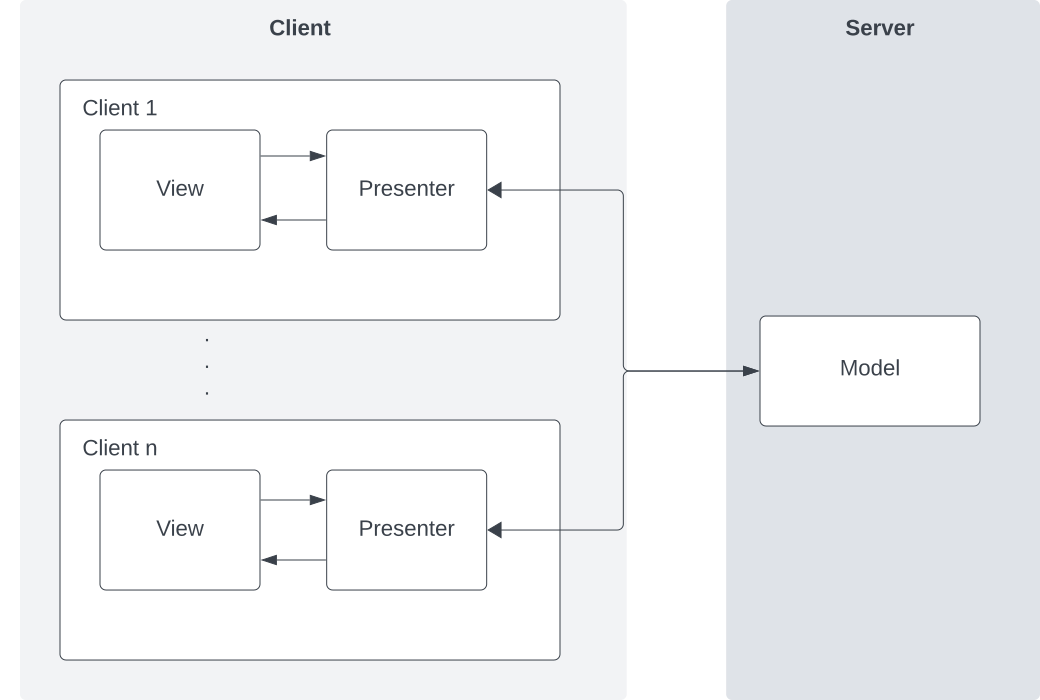
\includegraphics[scale=0.35]{chapters/Anhang/Präsenzphase/img/rmimvp}
    \caption{Das MVP-Architekturmuster in einer verteilten Anwendung. Das Model wird i.d.R. als \textit{remote object} realisiert, mit dem der Presenter kommuniziert.
    Wird auch der Presenter exportiert, ist das Model dazu in der Lage, die Presenter der Clients über entsprechende Schnittstellen direkt zu beeinflussen (in der Skizze über die \textit{bidirektionale} Verbindung Presenter - Model dargestellt (s. hierzu auch die Implementierung des Chat-Clients in \cite[349, Bild 6.12]{Oec22}). (Quelle: eigene)}
    \label{fig:rmimvp}
\end{figure}
